\chapter{Cataloguing the energetic contributions to the supramolecular assembly of \textit{p}-substituted \textit{N,N'}-diphenylureas and their organometallic derivatives in the solid state: a density functional theory approach}
\label{chap:cataloguing}

The following chapter was published in Crystal Growth and Design under authors Jenny W. Fothergill, Dr. Adam C. Colson, and Dr. Matthew D. King. My contributions to this paper were DFT calculations under the guidance of Dr. King, writing of the initial draft, and figure creation.

\section{Abstract}
Crystal engineering relies on the predictability of the elaborate interplay of cohesive and conformational energies driven by both intra- and intermolecular interactions of the constituent molecules. In an effort to better understand these influences on crystal packing of \textit{p}-substituted \textit{N,N'}-diphenylureas (\textit{p}DPUs) and organometallic derivatives, we present a detailed computational investigation of \textit{p}DPU species utilizing solid-state density functional theory (DFT), and demonstrate the applicability of predictive supramolecular synthons applied towards growth of related organometallic complexes. Dominant noncovalent interactions of \textit{p}DPUs can be tuned by altering the electron-withdrawing character of the \textit{p}-substituents. The strength of this electron-withdrawing nature governs the inclination of the molecules to form either dominant electrostatic or $\pi$-stacking intermolecular interactions in the crystal structure due to potential molecular conformational stabilization through intramolecular C-H$\cdot \cdot \cdot$O electrostatic interactions between \textit{ortho} phenyl hydrogens and the urea oxygen atoms. This propensity is also influenced by the symmetry of \textit{p}-substitutions in mono- and di-substituted DPUs. The results of the holistic DFT investigation show a relationship between gas-phase and solid-state conformations, and also presents evidence of mechanisms leading to deviations in predicted crystallization behaviors based on the balance of intra- and inter-molecular interactions. The foundational computational study was expanded to build on previous experimental and theoretical work involving zerovalent transition metal complexes in which \textit{p}-isocyanophenyl DPUs were appended with group IV metal carbonyl fragments. In this study, we synthesized an asymmetric analogue of the latter in which \textit{N}-(\textit{p}-isocyanophenyl)-\textit{N'}-phenylurea (\textit{p}CNHDPU) was appended to a Mo(CO)$_{5}$ metal carbonyl fragment, allowing us to associate the crystallization behaviors and interactions of organometallic DPU derivatives with those of simpler \textit{p}DPUs. It was observed that the supramolecular assembly of the organometallic complexes display similar predictive patterns, as well as additional complexities to molecular packing arising of the bulkier metal carbonyl substituents. An inclusive computational categorization of DPU-based systems in complement to experimental data will aid in the advancement of design rules for patterned crystal growth of DPU and related systems for the development of innovative materials having unique solid-state properties.

\section{Introduction}
The properties of supramolecular aggregates and molecular crystals may differ considerably from those of their isolated molecular constituents, and developing a deeper understanding of the noncovalent interactions that guide molecular assembly could contribute to advances in various applications, including the self-assembly of light-emitting diodes (LEDs), photovoltaic arrays, and field-effect transistors (FETs) \citep{Desiraju2007a, Corpinot2019a, Albrecht2007, Mukherjee2015a, Schneider2009, Yao2018}. The \textit{N,N'}-diphenylurea (DPU) moiety is a particularly versatile synthon for supramolecular assembly because it can participate in multiple types of noncovalent interactions. \textit{N,N'} diphenylureas bearing electron-donating functional groups can act as both hydrogen bond donors and acceptors, resulting in the formation of supramolecular ``ribbons'' or ``tapes'' (\autoref{fig:motifs}a) \citep{Custelcean2008, Etter1988a}. Alternatively, aromatic rings bearing electron-withdrawing functional groups can participate in $\pi$-$\pi$ interactions, resulting in the slip-stack packing of relatively planar \textit{N,N'} diphenylurea units, as depicted in \autoref{fig:motifs}b \cite{Yao2018}.  


%FIGURE 1 
\begin{figure}[h!]
    \centering
    
\includegraphics[width=0.8\linewidth]{figures/pub3/Picture1.png}
    \caption{Supramolecular motifs associated with \textit{N,N'}-diphenylurea compounds.}\label{fig:motifs}
\end{figure}

In addition to $\pi$-$\pi$ interactions, we have recently reported that $\pi$-urea interactions can facilitate the assembly of anisotropic molecular arrays in the solid state \citep{Millard2019a}. Organometallic DPUs prepared by tethering Mo(CO)$_{5}$ fragments to 1,3-bis(\textit{p}-isocyanophenyl)urea were observed to exhibit an unusual ladder-like packing motif consisting of alternating $\pi$-$\pi$ and urea-$\pi$ interactions. Intriguingly, solid state DFT calculations revealed that the cohesive contributions from the $\pi$-$\pi$ and urea-$\pi$ interactions to the total lattice energy were nearly equal in magnitude. This holistic computational treatment of lattice energy provided important insights into the subtleties of the intermolecular interactions governing molecular assembly in the solid state. The present work describes a more expansive computational effort to survey the lattice energies of DPU systems bearing electron-withdrawing functional groups and to identify the cohesive and conformational strain energy contributions to their overall lattice energies. Additionally, a mono-substituted Mo(CO)$_{5}$ derivative of the previously reported metal-bound 1,3-bis(\textit{p}-isocyanophenyl)urea was synthesized and crystallized to relate observed supramolecular behavior of these organometallic complexes with the predictability discerned from the explored \textit{p}DPUs. Ultimately, we anticipate that the findings presented in this work will inform the development of design rules for the patterned crystal growth of DPU-based systems.  

\section{Materials and Methods}
\subsection{Theoretical}

The DPU molecules selected for this study include 1,3-bis(\textit{p}-cyanophenyl)urea (\textit{p}CyDPU), 1-(\textit{p}-cyanophenyl)-3-(\textit{p}-nitrophenyl)urea (\textit{p}CyNDPU), 1,3-bis(\textit{p}-trifluoromethylphenyl)urea (\textit{p}CF$_{3}$DPU), 1-(\textit{p}-cyanophenyl)-3-phenylurea (\textit{p}CyHDPU), 1-(\textit{p}-nitrophenyl)-3-phenylurea (\textit{p}NHDPU), and 1-(\textit{p}-chlorophenyl)-3-phenylurea (\textit{p}ClHDPU), the crystal structures of which have previously been archived in the Cambridge Crystallographic Data Centre (\textit{p}CyDPU, 1554302; \textit{p}CyNDPU, 676835; \textit{p}CF$_{3}$DPU, 1554299; \textit{p}CyHDPU, 1554301; \textit{p}NHDPU, 676839; \textit{p}ClHDPU, 1554300) \citep{Groom2016a, Solomos2017a}. All DFT calculations were performed using the Crystal14 software package \citep{Dovesi2014b, Dovesi2016}. Calculations utilized a pairwise dispersion-corrected B3LYP-D2 density functional with the atom-centered triple-$\zeta$ basis with polarization functions, pob-TZVP, which is an Aldrich's triple-$\zeta$ basis set modified for solid-state calculations \citep{Becke1993c, Grimme2004a, Lee1988, Peintinger2013}. Dimer calculations used Ahlrich's valence triple-$\zeta$ basis \citep{Schafer1994, Schuchardt2007}. Atomic coordinates determined using single crystal X-ray diffraction were used as the initial geometry for the crystal structure optimization. The energy minimization allowed full relaxation of the atom positions within the constraints of the space group symmetry to a residual force of 10$^{-6}$ hartree. Shrinking factors of 3 (\textit{p}CF$_{3}$DPU), 4 (\textit{p}CyDPU, \textit{p}CyNDPU, \textit{p}NHDPU, \textit{p}ClHDPU), and 6 (\textit{p}CyHDPU) were used in defining the \textbf{k} point sampling of the density matrix in reciprocal space \citep{Gilat1972, Monkhorst1976a}. Corrections for basis set superposition error (BSSE) were performed using the counterpoise method \cite{Boys1970}. The lattice energy was calculated using the energy of the optimized crystal structure ($E_{cell}$) and the BSSE-corrected energy of a single molecule ($E_{moleculeBSSE}$) as follows:
\begin{equation}\label{elattice}
    E_{Lattice}=\frac{E_{cell}-Z \times E_{moleculeBSSE}}{Z}
\end{equation}
where $Z$ is the number of molecules in the unit cell. The strain energy of the crystal packing was calculated using the single point energies of a molecule extracted from the crystal structure ($E_{moleculeSP}$) and the energy of the molecule after geometry optimization ($E_{moleculeopt}$) as follows:
\begin{equation}\label{estrain}
    E_{strain} = E_{moleculeSP} - E_{moleculeopt}
\end{equation}
The cohesive energy was calculated as follows:
\begin{equation}\label{ecohesive}
    E_{cohesive} = E_{lattice} - E_{strain}
\end{equation}
Interaction energies for the dimer structures were calculated using single-point energies of dimers extracted from the optimized crystal structure ($E_{dimer}$), along with BSSE-corrected molecular single-point energies as follows:
\begin{equation}\label{einteraction}
    E_{interaction} = E_{dimer} - 2 \times E_{moleculeBSSE}	
\end{equation}

\subsection{Experimental}
\subsubsection{General Considerations}
All synthetic operations were carried out under a nitrogen atmosphere using standard Schlenk techniques to exclude moisture and oxygen. Nitrogen was prepurified by passage through columns of activated copper catalyst (BASF PuriStar R3-11G) and molecular sieves (RCI-DRI 13X). Glassware was dried in an oven at 130 °C, assembled while hot, and allowed to cool under reduced pressure. All solvents were dried according to published procedures and degassed with nitrogen prior to use. Mo(CO)$_{6}$ (Acros, 98\%), trimethylamine \textit{N}-oxide dihydrate (Beantown Chemical, 98\%), and phenyl isocyanate (Acros, 99\%) were used as received without further purification. 4-Isocyanophenylamine was prepared according to literature procedures and sublimed prior to use \cite{Heinze2003}. Infrared spectra were obtained using a Thermo Scientific Nicolet iS5 FTIR spectrometer equipped with a 0.2 mm BaF$_{2}$ liquid cell. $^{1}$H and $^{13}$C NMR data were recorded on a 600 MHz Bruker AVANCE III spectrometer. Electrospray ionization mass spectrometry (ESI-MS) was carried out using a Bruker HCTultra CTD II spectrometer in negative ion mode. CH$_{3}$CN solutions of analytes were treated with the tetrabutylammonium salts of chloride and nitrate prior to injection into the mass spectrometer. Elemental analyses were performed by Atlantic Microlab, Inc in Norcross, GA, USA.

\subsubsection{Synthesis of \textit{N}-(\textit{p}-isocyanophenyl)-\textit{N'}-phenylurea (\textit{p}CNHDPU)} \textit{p}-Isocyanophenylamine (318 mg, 2.69 mmol) and phenyl isocyanate (300 mg, 2.52 mmol) were dissolved in 20 mL of CH$_{3}$CN. The reaction mixture was heated at reflux for three hours, after which the solvent was removed under reduced pressure. The solid residues were washed with toluene followed by hexanes and dried under reduced pressure. The product was isolated as a pale yellow solid (433 mg, 72\% yield). IR (CH$_{2}$Cl$_{2}$, cm$^{-1}$): $\nu_{CN}$ 2064 (vs). $^{1}$H NMR (CD$_{3}$CN, 20 °C): $\delta$ 7.05 (t, \textit{J} = 7.41 Hz, 1H, Ar H), 7.31 (t, \textit{J} = 8.15 Hz, 2H, Ar H), 7.37 (m, 3H), 7.44 (d, \textit{J} = 7.61 Hz, 2H, Ar H), 7.53 (d, \textit{J} = 8.59 Hz, 2H Ar H), 7.55 (br s, 1H, NH). $^{13}$C NMR (CD$_{3}$CN, 20 °C): $\delta$ 117.3, 119.0, 122.9, 127.1, 128.8, 139.1, 140.7, 152.3, 163.4, 206.5. MS(ESI): \text{m/z} 272 [M + Cl$^{-}$]$^{-}$, 299 [M + NO3$^{-}$]$^{-}$. Anal. Calcd for C$_{14}$H$_{11}$N$_{3}$O: C, 70.87; H, 4.67; N, 17.71. Found: C, 70.58; H, 4.63; N, 17.91. 

\subsubsection{Synthesis of Mo(CO)$_{5}$(\textit{p}CNHDPU)} Mo(CO)$_{6}$ (556 mg, 2.11 mmol) and \textit{p}CNHDPU (500 mg, 2.11 mmol) were dissolved in 25 mL of tetrahydrofuran (THF), and a dropping funnel charged with trimethylamine \textit{N}-oxide dihydrate (233 mg, 2.10 mmol), THF (10 mL), and methanol (10 mL) was attached to the reaction flask, the contents of which were added dropwise to the reaction mixture over the course of one hour. The mixture was magnetically stirred for six hours at room temperature, after which the solvents were removed under reduced pressure. The residues were extracted with ethyl acetate, filtered to remove insoluble impurities, and adsorbed onto silica gel. Mo(CO)$_{5}$(\textit{p}CNHDPU) was isolated by column chromatography using silica gel as the stationary phase and a mixed solvent system as eluent (5:4:1 vol. eq. CH$_{2}$Cl$_{2}$, hexanes, and ethyl acetate). The chromatographic fractions were dried under reduced pressure and the residues dissolved in \textit{N,N'}-dimethylformamide (DMF). Slow titration of the DMF solution with distilled water produced colorless crystalline needles (606 mg, 61\% yield). IR (CH$_{2}$Cl$_{2}$, cm$^{-1}$): $\nu_{CN}$ 2143 (m), $\nu$CO 2063 (s), 1956 (vs). $^{1}$H NMR (CD$_{3}$CN, 20 °C): $\delta$ 7.05 (t, 1H, Ar-H, \textit{J} = 7.41 Hz), 7.31 (t, 2H, Ar-H, \textit{J} = 8.15 Hz), 7.40 (m, 3H), 7.45 (d, \textit{J} = 7.61 Hz, 2H, Ar H), 7.55 (d, \textit{J} = 8.59 Hz, 2H Ar H), 7.61 (br s, 1H, N-H). $^{13}$C NMR (CD$_{3}$CN, 20 °C): $\delta$ 119.3, 127.2, 140.4, 151.8, isocyanide and adjacent ipso carbons not observed. MS(ESI): \text{m/z} 510 [M + Cl$^{-}$]$^{-}$, 537 [M + NO3$^{-}$]$^{-}$. Anal. Calcd for C$_{19}$H$_{11}$MoN$_{3}$O$_{6}$: C, 48.22; H, 2.34; N, 8.88. Found: C, 48.16; H, 2.26; N, 8.98.

\section{Results and Discussion}
The crystal structures of several \textit{p}-substituted DPUs were acquired from the Cambridge Crystallographic Database, which represent a diverse cross-section of DPU derivatives to compare preferred molecular conformations, crystal packing configurations, and interaction energies as a function of the electron-withdrawing nature of the \textit{p}-substituents. The systems studied were 1,3-bis(\textit{p}-cyanophenyl)urea (\textit{p}CyDPU), 1-(\textit{p}-cyanophenyl)-3-(\textit{p}-nitrophenyl)urea (\textit{p}CyNDPU), 1,3-bis(\textit{p}-trifluoromethylphenyl)urea (\textit{p}CF$_{3}$DPU), 1-(\textit{p}-cyanophenyl)-3-phenylurea (\textit{p}CyHDPU), 1-(\textit{p}-nitrophenyl)-3-phenylurea (\textit{p}NHDPU), and 1-(\textit{p}-chlorophenyl)-3-phenylurea (\textit{p}ClHDPU) (\autoref{fig:structures}). The selected structures offer both mono- and di-\textit{para}-substituted DPUs having electron withdrawing substituents of varying magnitudes.


% FIGURE 2 
\begin{figure}[h!]
    \centering
    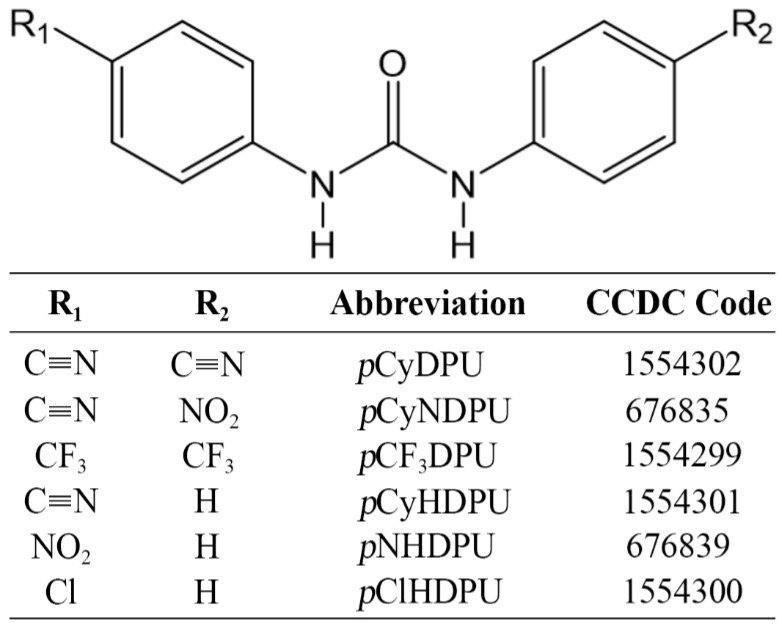
\includegraphics[width=0.8\linewidth]{figures/pub3/Picture2.jpg}
    \caption{Chemical structures of \textit{p}DPUs examined in this study.}\label{fig:structures}
\end{figure}

The implications of the \textit{p}DPU molecular structures is that they may facilitate the dominant interactions driving crystal packing formation. Information on molecular structure can therefore provide predictive insight towards patterned crystal growth and engineering. There exists an interplay between intramolecular forces, intermolecular forces, and molecular conformational strain that govern how each DPU will behave in the gas and solid states. In the crystalline solid, any molecular DPU conformation can participate in the urea ribbon motif, but planar molecules are favored for $\pi$-stacking interactions. In instances of DPU planarity, steric hindrances of adjacent rings prevent the formation of the hydrogen-bonded urea ribbon motif and rely on stabilization through $\pi$-$\pi$ interactions. However, ring substituents may contribute to additional lattice stabilization by forming hydrogen bonds with the available urea moieties. In order for a DPU to achieve planarity, the electrostatics of the ring must be altered through addition of electron-withdrawing substituent groups at the \textit{para} position. Such additions result in a coupled withdrawal of charge density at the \textit{ortho} position, thus generating greater positive charge localized on the \textit{ortho}-hydrogens. Although not a ``true'' hydrogen bond, the electrostatic interaction between the \textit{ortho}-hydrogen on the aromatic ring and the urea oxygen may facilitate stabilization of a co-planar aryl conformation. This favorable electrostatic interaction is countered by the repulsion between the opposite \textit{ortho}-hydrogen of the same ring and the urea hydrogen. The magnitude of the hydrogen bonding is greater than that of this H-H repulsion, which can therefore be overcome only through structural addition of strong electron-withdrawing groups. The favored \textit{molecular} conformation ultimately affects the \textit{crystal} packing configuration, and the degree of DPU planarity and its ability to form stabilizing $\pi$-$\pi$ interactions in the crystal phase is dependent on the magnitude of the electron-withdrawing character of the \textit{p}-substituent group(s).

Contained in the investigated structures are the ring substituents chloro, cyano, trifluoromethyl, and nitro groups. From our single-molecule DFT calculations, Mulliken charges of the electron-withdrawing groups were determined and ranked as NO$_{2}$ > Cl > CN > CF$_{3}$ in terms of net negative group charge (averages of -0.54, -0.23, -0.13, -0.10, respectively). The propensity to form planar molecular structures, and therefore encourage $\pi$-$\pi$ stacking motifs in the crystal structure, is a result of the withdrawal of electron density from the phenyl ring and shifting electron density away from the \textit{ortho}-H, thereby increasing the strength of the \textit{o}-H$\cdot \cdot \cdot$O$_{urea}$ stabilizing intramolecular interaction. Evident by the single-molecule structural optimizations shown in \autoref{fig:geom-opt}, the strength of the electron-withdrawing character at the \textit{para} position has a notable effect on preferred molecular configuration. Non-substituted DPU optimizes with the phenyl groups twisted $\sim$40° from the urea N-C-N plane due to repulsion between the \textit{o}-H and H$_{urea}$, yielding H$\cdot \cdot \cdot$H distances of 2.29 \AA. These repulsive forces are balanced by the weak interactions between the adjacent \textit{o}-H and the O$_{urea}$ at 2.40 \AA. The addition of \textit{p}-substitutions to the DPU molecular structures alters the electron density at the important \textit{ortho} position and, hence, the ring orientations. The di-substituted \textit{p}CyNDPU contains the strongest electron-withdrawing groups, and the resulting optimized structure is nearly planar due to the increase interaction strength between the \textit{o}-H and the O$_{urea}$. The preferred molecular orientation has nearly equivalent \textit{o}-H$\cdot \cdot \cdot$O$_{urea}$ and \textit{o}-H$\cdot \cdot \cdot$H$_{urea}$ separations of 2.20 and 2.21 \AA, respectively. Examination of the remaining molecule structures reveals that deviation from planarity is increased. In the case of \textit{p}CF$_{3}$DPU, which has the weakest electron withdrawing character, the resulting structure is nearly that of the non-substituted DPU structure with \textit{o}-H$\cdot \cdot \cdot$O$_{urea}$ and \textit{o}-H$\cdot \cdot \cdot$H$_{urea}$ distance of 2.37 and 2.28 \AA, respectively. 


% FIGURE 3  
\begin{figure}[h!]
    \centering
    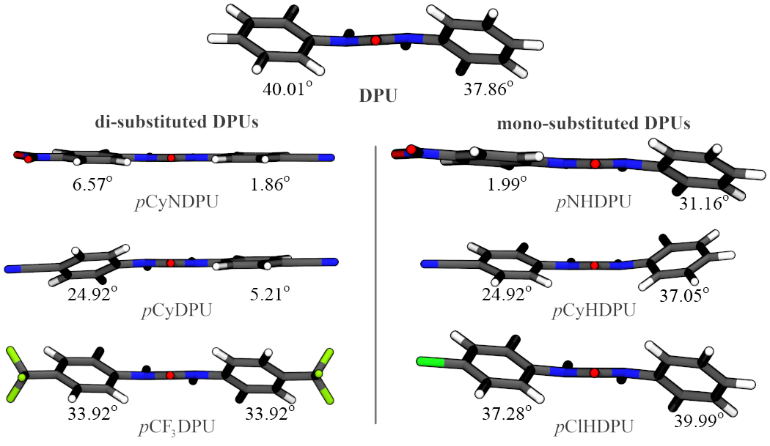
\includegraphics[width=0.8\linewidth]{figures/pub3/Picture3.png}
    \caption{Single-molecule geometry optimizations of \textit{p}DPUs.}\label{fig:geom-opt}
\end{figure}

The trend in ring planarity as a function of the electron-withdrawing character of the ring substituent is clear looking at the three optimized mono-substituted DPU molecules. The \textit{o}-H$\cdot \cdot \cdot$O$_{urea}$ distances with respect to the \textit{p}-substituted ring were 2.19, 2.28, and 2.38 \AA for the NO$_{2}$, CN, and Cl substitutions, respectively (2.21, 2.26, and 2.30 \AA for the \textit{o}-H$\cdot \cdot \cdot$H$_{urea}$). The relative orientation of the non-substituted ring was not significantly different between each of the structures, and corresponded to the structural parameters observed for the non-substituted DPU structural optimization. However, slight variations in the \textit{o}-H$\cdot \cdot \cdot$O$_{urea}$ distances were calculated due to the overall molecular redistribution of electron density resulting from the single ring substitution. These distances with respect to the non-substituted ring were calculated to be 2.34, 2.39, and 2.43 \AA for the NO$_{2}$, CN, and Cl substitutions, respectively (2.27, 3.33, and 2.30 \AA for the \textit{o}-H$\cdot \cdot \cdot$H$_{urea}$).

In molecular crystals systems, the relationship of packing forces and conformational strain energies often results in deviations between molecular structures observed in the solid phase and that of the optimized single-molecule `gas phase' orientation. These structural deviations can sometimes be significant such that molecules cannot be treated as rigid building blocks in the construction of thermodynamically stable crystal structures. Optimization of lattice energy during crystal growth depends upon maximization of stabilizing intermolecular interactions while minimizing distortion of the molecules from their most stable molecular conformation. It is the relative strengths of these intra- and inter-molecular forces that ultimately determine the crystalline configuration of organic molecules. As such, the single-molecule structures of the \textit{p}DPUs were compared to those taken in their respective crystal structures in order to better understand the influence of preferred molecular conformation of crystal packing assembly. In the case of \textit{p}DPUs, two primary intermolecular interactions are present: hydrogen bonding through the urea moiety and $\pi$-$\pi$ interactions between phenyl rings. In the formation of a stable crystalline packing orientation, the system must either maintain the preferred molecular structure or overcome the magnitude of the intramolecular interactions within the \textit{p}DPU molecules.

The general packing assembly of the \textit{p}DPUs are shown in \autoref{fig:packing}. Although all crystal structures are composed of molecules containing the DPU motif, the crystal structures are quite different depending on the dominant supramolecular interactions. The molecular orientation of di-substituted DPUs as they are found in the crystal structure generally follow those of the single molecule optimizations. Stabilization of the planar molecular structures in the cases of \textit{p}CyNDPU and \textit{p}CyDPU through \textit{o}-H$\cdot \cdot \cdot$O$_{urea}$ interactions, and inversely the lack of electrostatic stabilization through the weakly electron withdrawing \textit{p}-substituents of \textit{p}CF$_{3}$DPU, provides the `rigid' building blocks for crystalline assembly. Preferentially planar molecules are likely to adhere to a $\pi$-stacking crystal orientation, and those lacking robust \textit{o}-H$\cdot \cdot \cdot$O$_{urea}$ interactions adopt urea hydrogen-bonding ribbon motif in the solid-state. Given the stability afforded by dominant intramolecular interactions, in this case the \textit{o}-H$\cdot \cdot \cdot$O$_{urea}$ interactions, reliable predictions can be made on the molecular configurations likely to be observed in the solid phase. The intricacies of the crystalline conformation also depend on other thermodynamic factors and the ability of the substituents to form additional stabilizing interaction with neighboring molecules. Take for example the \textit{p}CyNDPU and \textit{p}CyDPU crystal systems. Even though both molecules adopt a planar molecular conformation in the crystal structure, the mechanism of stacking of these planar molecules differs between the two. The \textit{p}CyDPU molecule forms continuous chains stabilized through $\pi$ - $\pi$ interactions, while \textit{p}CyNDPU forms paired molecular $\pi$ - $\pi$ stacking and lacks a continuous chain resulting from this type of interaction. The reason is the ability of the \textit{p}CyNDPU to also form hydrogen bonds with neighboring molecules through adjacent -NO$_{2}$ and -CN substituents. This takes advantage of not only the spatial advantage of stacking flat molecular building blocks, but also enables strong contacts to be made between neighboring molecules. The result of this is the maximization of crystal density and minimization of total lattice energy by forming the strongest possible ensemble of favorable molecular interactions.  


% FIGURE 4 
\begin{figure}[h!]
    \centering
    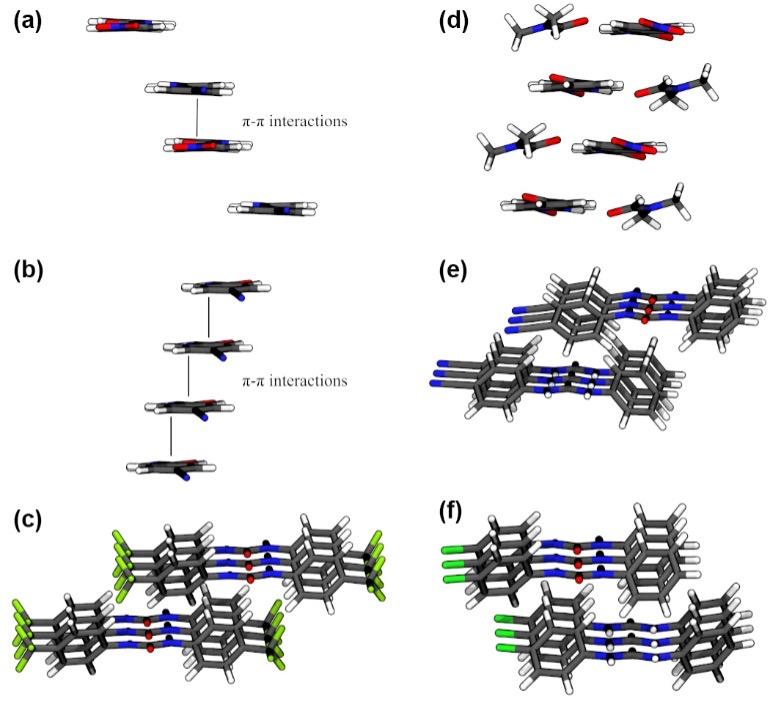
\includegraphics[width=0.8\linewidth]{figures/pub3/Picture4.jpg}
    \caption{Primary packing orientations within the \textit{p}DPU crystal structures of \textbf{\textbf{(a)}} \textit{p}CyNDPU, \textbf{(b)} \textit{p}CyDPU, \textbf{(c)} \textit{p}CF$_{3}$DPU, \textbf{(d)} \textit{p}NHDPU, \textbf{(e)} \textit{p}CyHDPU and \textbf{(f)} \textit{p}ClHDPU.}\label{fig:packing}
\end{figure}

The situation becomes more complex for mono-substituted DPUs where only half the molecule may experience stabilizing intramolecular \textit{o}-H$\cdot \cdot \cdot$O$_{urea}$ contacts. In this case, the intricate balance of intra- and intermolecular forces guiding crystal packing configurations leans towards the dominant crystalline intermolecular interactions. Energetic favorability is gained through disruption of the molecular structure and subsequent optimization of molecular packing rather than maintaining the gas-phase molecular orientation. Most demonstrable in the crystal systems examined is that of \textit{p}CyHDPU in comparison to the di-substituted \textit{p}CyDPU. Mono-substitution of the electron-withdrawing -CN group is not sufficient to preserve a planar molecular orientation in the crystal phase. The resulting crystal structure contains \textit{p}CyHDPU molecules in the preferred packing efficiency that involves the urea ribbon motif, thus overcoming the intramolecular interactions resulting in the partially planar gas-phase orientation imposed by the electron-withdrawing -CN substituent. Also a factor is the reduced ability to form stabilizing hydrogen bonding between the -CN \textit{p}-substituents and the urea hydrogens an efficient manner due to spatial constraints and reduced molecular symmetry.

Noteworthy disparity in crystallization behavior is also discerned in \textit{p}NHDPU. This molecule forms a solvate crystal structure in which DMF solvent molecules are intercalated into the co-crystallized system at a 1:1 ratio with \textit{p}NHDPU. The energetic balance is addressed by allowing \textit{p}NHDPU to maintain their preferred planar molecular orientations afforded by the strong electron-withdrawing character of the -NO$_{2}$ substituent. Without the ability for NO$_{2}$ to form additional stabilizing intermolecular hydrogen bonds with neighboring molecules in a spatially favorable manor, it becomes advantageous for co-crystallization with DMF as opposed to a geometrically strained $\pi$-stacking configuration. Additional stabilization energy is acquired through hydrogen bonding of the DMF oxygen atom with the urea hydrogens of \textit{p}NHDPU. The reduction in molecular symmetry between the di-substituted \textit{p}CyNDPU and mono-substituted \textit{p}NHDPU prevents an efficient packing configuration to enable the hydrogen bonding between \textit{p}-substituents and urea moieties. Interestingly, there is also no $\pi$-stacking interactions stabilizing the crystal structure, which would be expected in systems containing co-planar phenyl groups. The limitations in options for hydrogen bonding within the crystal to overcome the intramolecular forces, and the associated limitations in packing configurations having one planar and one non-planar phenyl orientation, provide a more favorable environment for solvent inclusion in the thermodynamically stable \textit{p}NHDPU crystal structure. The molecules are able to maintain their planar configuration while achieving a favorable crystal packing density through the solvent inclusion.

Solid-state DFT calculations where performed to evaluate the balance of interactions leading to the desired crystalline conformations observed for the various \textit{p}DPUs. The lattice energy provides a measure of the driving force for the molecules to form in the solid state. In order to obtain an optimal lattice energy, the system must be able to form favorable intermolecular interactions while being counteracted by the necessity to overcome intramolecular attractions, thus creating an unfavorable molecular strain energy that is compensated by a more advantageous lattice energy. The results of energy calculations of the \textit{p}DPU crystal systems are provided in \autoref{tab:dpu-energies} and expressed in terms of lattice energy broken down into cohesive and molecular conformational strain energies. Also tabulated are the interaction energies between dimers extracted from the crystal structures that contain the desirable supramolecular interaction motif, i.e. hydrogen-bonded chain or $\pi$-stacking, exhibited in each crystal system. Although many favorable interactions for crystal assembly may be present in a particular system, only the dominant intermolecular interactions were examined. This energetic component is isolated to provide additional information that connects the single-molecule and crystalline conformations of the constituent molecules. In the case of \textit{p}NHDPU, for which DMF solvent co-crystallizes at a 1:1 ratio, the prominent dimer energetic contribution is that of the hydrogen bonding between the DMF oxygen and the \textit{p}NHDPU urea hydrogens. Mulliken population analysis was performed for each system to analyze partial charges on the O$_{urea}$, \textit{o}-H, and \textit{o}-C atoms of the crystalline \textit{p}DPU structures (\autoref{tab:mulliken}). The results show that when the \textit{p}-substituted groups are sufficiently electron-withdrawing, the hydrogens in the \textit{ortho} position are more positively charged and can therefore interact more strongly with O$_{urea}$. This is best demonstrated by comparing the symmetric \textit{p}CyDPU and \textit{p}CF$_{3}$DPU molecules, for which the stronger electron withdrawing group, -CN, produced a net positive charge of +0.090 at the \textit{o}-H's, whereas CF$_{3}$ substitution yielded only a charge of +0.056 on these atoms. This seemingly small difference in atomic charge is sufficient to greatly influence the intramolecular structure and the resulting primary intermolecular motif exhibited in the crystal structure. 


%TABLE 1 
\begin{table}[]
\centering
\caption{Calculated lattice, cohesive, strain, and dimer energies for \textit{p}DPU crystal structures. Energies provided in units of kcal mol$^{-1}$.} \label{tab:dpu-energies}
\begin{tabular}{lrrrr}
\textbf{Complex} & $E_{Lattice}$ & $E_{Cohesive}$ & $E_{Strain}$ & $E_{Dimer}$ \\ \hline
\multicolumn{2}{l}{\textbf{di-substituted}} &  &  &  \\
\textit{p}CyDPU & -72.83 & -94.78 & 21.95 & -49.07 \\
\textit{p}CyNDPU & -74.60 & -97.58 & 22.98 & -57.17 \\
\textit{p}CF$_{3}$DPU & -76.72 & -105.46 & 28.74 & -73.64 \\
\multicolumn{2}{l}{\textbf{mono-substituted}} &  &  &  \\
\textit{p}CyHDPU & -65.17 & -87.39 & 22.22 & -57.27 \\
\textit{p}NHDPU & -90.87 & -112.70 & 21.83 & -42.49$^{a}$ \\
\textit{p}ClHDPU & -66.39 & -88.55 & 22.15 & -57.38 \\ \hline
\multicolumn{5}{l}{$^{a}$\textit{p}NHDPU:DMF dimer interaction energy}
\end{tabular}
\end{table}


%TABLE 2 
\begin{table}[]
\centering
\caption{Mulliken population analysis of partial charges on the O$_{urea}$, \textit{o}-H, and \textit{o}-C atoms in \textit{p}DPUs (reported as elementary charge units). The average charges are reported for di-substituted DPUs, and both substituted and non-substituted phenyl groups are reported for mono-substituted DPUs. The phenyl ring with the electron withdrawing group (EWG) or hydrogen (H) at the \textit{para} position are denoted.} \label{tab:mulliken}
\begin{tabular}{lrrcrcr}
\textbf{di-substituted} & \multicolumn{2}{r}{\textbf{O$_{urea}$}} & \multicolumn{2}{c}{\textbf{\textit{o}-H}} & \multicolumn{2}{c}{\textbf{\textit{o}-C}} \\ \hline
\textit{p}CyDPU & \multicolumn{2}{r}{-0.73} & \multicolumn{2}{c}{+0.09} & \multicolumn{2}{c}{-0.05} \\
\textit{p}CyNDPU & \multicolumn{2}{r}{-0.73} & \multicolumn{2}{c}{+0.09} & \multicolumn{2}{c}{-0.05} \\
\textit{p}CF$_{3}$DPU & \multicolumn{2}{r}{-0.75} & \multicolumn{2}{c}{+0.06} & \multicolumn{2}{c}{-0.00} \\ \hline
\textbf{mono-substituted} & \textbf{O$_{urea}$} & \multicolumn{2}{r}{\textbf{\textit{o}-H   (EWG)}} & \textbf{\textit{o}-H   (H)} & \multicolumn{1}{r}{\textbf{\textit{o}-C (EWG)}} & \textbf{\textit{o}-C (H)} \\ \hline
\textit{p}CyHDPU & -0.77 & \multicolumn{2}{r}{+0.06} & +0.04 & \multicolumn{1}{r}{-0.01} & +0.01 \\
\textit{p}NHDPU & -0.74 & \multicolumn{2}{r}{+0.09} & +0.07 & \multicolumn{1}{r}{-0.06} & -0.04 \\
\textit{p}ClHDPU & -0.75 & \multicolumn{2}{r}{+0.05} & +0.05 & \multicolumn{1}{r}{+0.00} & -0.01 \\ \hline
\end{tabular}
\end{table}


The lattice energies are similar among the di-substituted \textit{p}DPU structures, with a slight increase in stabilization energy as the strength of the electron-withdrawing \textit{p}-substituent decreases (\autoref{tab:dpu-energies}). The same trend is observed in the dimer energies and is much more pronounced, suggesting that the hydrogen bonded urea ribbon motif is considerably more stable than the primary $\pi$-stacking interactions exhibited in the \textit{p}CyDPU and \textit{p}CyNDPU crystal packing (\autoref{fig:packing}). However, in order to achieve hydrogen bonding between urea moieties of adjacent molecules, the molecules must undergo large conformational changes. Accompanied with this change is a substantial increase in conformational strain energy. For instance, the \textit{p}CyDPU and \textit{p}CyNDPU molecules exhibited comparable conformational strain energies of 21.95 and 22.98 kcal mol$^{-1}$, whereas \textit{p}CF$_{3}$DPU revealed a larger 28.74 kcal mol$^{-1}$ due to the molecular deformation required to attain the urea ribbon motif. The strain energy of the planar \textit{p}CyDPU and \textit{p}CyNDPU molecules would be necessarily much higher to achieve an analogous ribbon hydrogen bonding pattern since more energy would be required to break their stronger \textit{o}-H$\cdot \cdot \cdot$O$_{urea}$ contacts. It is therefore more energetically favorable for the planar \textit{p}CyDPU and \textit{p}CyNDPU configurations to maintain intramolecular \textit{o}-H$\cdot \cdot \cdot$O$_{urea}$ contacts while minimizing conformational strain energy. The tradeoff of energy contributions yields comparable lattice energies for each of the di-substituted DPU crystal structures. 

Of the molecular crystals examined in this study, only \textit{p}CyDPU and \textit{p}CyNDPU display evidence of $\pi$-stacking (\autoref{fig:slip-stack}). The symmetrically substituted \textit{p}CyDPU exhibits isotropic molecular stacking, forming contiguous $\pi$-stacked arrangements in the solid state, whereas the $\pi$-stacked \textit{p}CyNDPU molecular dimers exist in orientations inverted to one another. This difference nonetheless yields comparable distances between ring centroids of 3.76 and 3.83 \AA, respectively. Energy calculations show the \textit{p}CyNDPU dimer interaction to be more favorable by 8.1 kcal mol$^{-1}$ due to added constructive interactions primarily between the \textit{o}-H and N$_{urea}$ of adjacent DPU molecules. The variations in relative orientations and overall packing configurations are accounted for by the additional hydrogen bonding interactions available between \textit{p}-substituents and the DPU urea group in the crystal structures. 


%FIGURE 5 
\begin{figure}[h!]
    \centering
    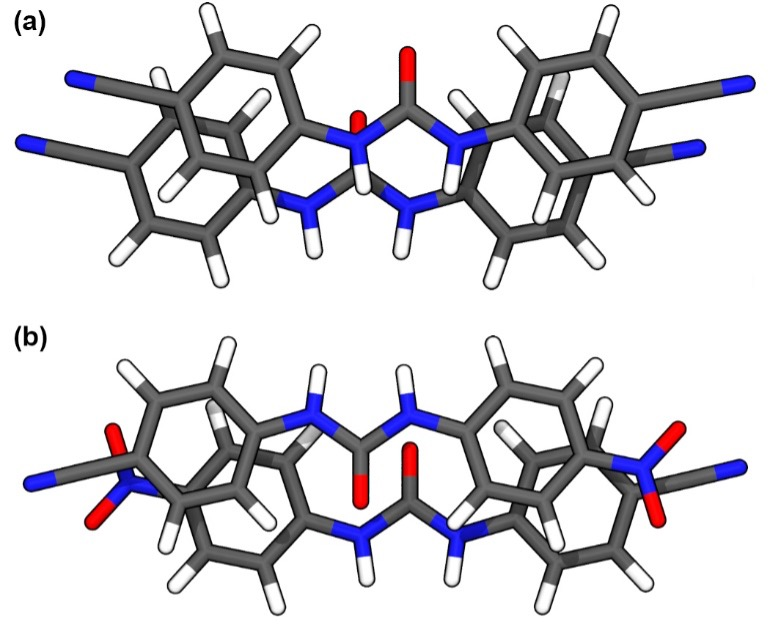
\includegraphics[width=0.8\linewidth]{figures/pub3/Picture5.jpg}
    \caption{\textbf{\textbf{(a)}} Top view of \textit{p}CyDPU dimer showing isotropic slipped $\pi$-stacking motif. The distance between the ring centroids is 3.76 \AA. \textbf{(b)} 	Top view of \textit{p}CyNDPU dimer showing slipped $\pi$-stacking motif, with a distance between ring centroids of 3.83 \AA in the crystal structure.}\label{fig:slip-stack}
\end{figure}

The most favorable lattice energy is observed in \textit{p}NHDPU. The dominant interaction in this crystal is hydrogen bonding between the urea hydrogens and the DMF oxygen. The molecule remains moderately planar allowing the crystal packing to adopt a herringbone stacking pattern. Although the planar conformation of \textit{p}NHDPU has the potential for $\pi$-stacking, the distance between the ring centroids (7.39 \AA) in the crystal structure is too great to expect that orbital overlap facilitates the crystal self-assembly. Despite the most favorable lattice energy, the weakest calculated primary interaction energy was between \textit{p}NHDPU and the co-crystallized DMF solvent. This was not surprising given the relatively small size of the DMF molecule and that the hydrogen bonding interaction between \textit{p}NHDPU and DMF is likely not as strong as those in structures with the urea ribbon motif since the DMF molecule will exhibit more thermal motion, whereas the urea ribbon in stabilized on both sides by the ribbon-like hydrogen bond network. However, the additional spatial freedom afforded by the inclusion of the smaller DMF molecules allows the crystal system to adopt the more energetically favorable herringbone packing configuration. 

The least favorable lattice energy is observed in the asymmetric \textit{p}CyHDPU which crystallizes according to the urea ribbon motif. The calculated lattice energy was -65.17 kcal mol$^{-1}$, in contrast to that of \textit{p}NHDPU of -90.87 kcal mol$^{-1}$. This raises the question as to why additional thermodynamic stability could not be achieved by \textit{p}CyHDPU through the formation of a DMF solvate as did its \textit{p}NHDPU counterpart. Inspection of the stabilizing partial charges on the \textit{o}-H atoms and the calculated strain energies of the two molecules suggests that considerable energy would be required for the \textit{p}CyHDPU molecule to adapt to a planar configuration in the crystalline configuration. The additional conformational strain energy needed to force this configuration would outweigh the stabilization energy gained by incorporating DMF solvent molecules into the crystal structure. One must also consider the nucleation and growth processes involved in crystallization. The DMF-\textit{p}NHDPU dimer interaction of -42.49 kcal mol$^{-1}$ is much weaker than that of the \textit{p}CyHDPU dimer of -57.27 kcal mol$^{-1}$. The stronger interaction of the \textit{p}CyHDPU dimer likely drives the contiguous kinetic growth of the crystal, whereas the combination of DMF stabilization and the inclination to conserve the planar intramolecular structure of \textit{p}NHDPU drives the thermodynamically favorable crystallization of the DMF-\textit{p}NHDPU solvate, even though the crystal structure lacks any obvious intermolecular interactions constructively leading to the auspiciously high lattice energy. 

Comparing structural similarities/disparities of those DPUs forming the urea ribbon motif, i.e. \textit{p}CF$_{3}$DPU, \textit{p}CyHDPU, and \textit{p}ClHDPU, two primary ring orientations are observed (\autoref{fig:ribbon-angle}). In order to achieve the ribbon hydrogen bonding pattern, the rings substituents must deviate from planarity. The \textit{p}CF$_{3}$DPU and \textit{p}ClHDPU have isostructural molecular conformations in their respective crystal structures. The ring substituent groups are twisted in opposite directions in relation to the urea moiety at plane angles formed between phenyl rings of 83.90° and 90.77°, respectively. The \textit{p}CyHDPU molecule adopts a different orientation in which the rings are rotated in the same direction in relation to the urea groups, possibly driven by the stronger electron-withdrawing character of the -CN group maintaining a higher degree of the \textit{o}-H$\cdot \cdot \cdot$O$_{urea}$ contact within the molecule. The resulting angle between phenyl planes was 142.58°. The differences observed in the DPUs are again the balance of intra- and intermolecular forces guiding the crystal formation, with variations in phenyl orientations resulting from the system pushing for optimal packing density through intermolecular interactions while preserving favorable intramolecular stabilization.   


% FIGURE 6 
\begin{figure}[h!]
    \centering
    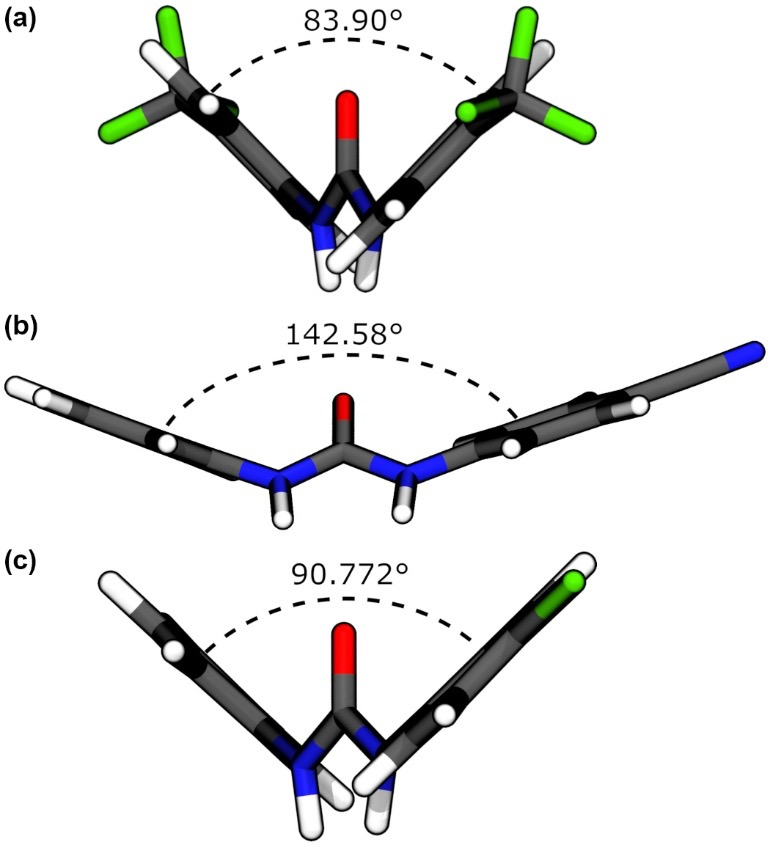
\includegraphics[width=0.8\linewidth]{figures/pub3/Picture6.jpg}
    \caption{Angle between ring planes in DPU structures crystallizing according to the urea ribbon motif: \textbf{(a)} \textit{p}CF$_{3}$DPU, \textbf{(b)} \textit{p}CyHDPU, and \textbf{(c)} \textit{p}ClHDPU.}\label{fig:ribbon-angle}
\end{figure}

The underlying motivation to investigate the intricacies of the crystal structures of \textit{p}-substituted DPUs comprises the interest of acquiring a broader understanding of how molecular structure, intra- and intermolecular interactions, and packing forces govern the organization of molecular solids. Progression of crystal engineering capabilities to direct the organization of molecular solids according to desired structural motifs requires the knowledge of not only the easily discernable intermolecular interactions, but also the subtle interactions that may exist within a molecule or that may be exposed following crystallization---many of which are often unexpected. This holds true for many crystal systems of related molecular species. Our interest in \textit{p}DPUs originates from our current developmental endeavors of low- and zerovalent transition metal carbonyl complexes incorporating \textit{p}-substituted \textit{N,N'}-diarylurea moieties as a facilitating agent for supramolecular chemistry and crystal engineering of advanced materials. The multiple supramolecular motifs made accessible by such DPUs offers much versatility in the generation of novel organometallic structures and functional materials.

We recently detailed the multifaceted interactions found in the crystal structures of organometallic complexes containing 1,3-bis(\textit{p}-isocyanophenyl)urea tethered to M(CO)$_{5}$ fragments (M = Cr, Mo, and W) via isocyanide linkages (\autoref{fig:solid-state-packing}). The coordination of bulky metal carbonyl fragments to the DPU scaffold introduced additional layers of complexity in that significant steric effects would expectedly influence the crystal packing configuration and the observed interaction motifs. The binuclear organometallic complexes were observed to pack into ladder-like anisotropic arrays in the solid state. Crystallographic and computational evidence suggested that the observed packing motif could be attributed to a combination of intermolecular $\pi$-$\pi$ and urea-$\pi$ interactions. Intriguingly, the magnitude of the unconventional urea-$\pi$ interactions was nearly equivalent to the familiar $\pi$-$\pi$ stacking motif, with respective cohesive energies of urea-$\pi$ and $\pi$-$\pi$ dimers calculated at -111.64 and -118.43 kcal mol$^{-1}$. The strength of the urea-$\pi$ interactions was explained through comprehensive analysis of electrostatics and favorable HOMO/LUMO overlap of the dimer complexes. Notable structural similarities of the carbonyl complexes with the \textit{p}-substituted DPUs presented in this study are that of ring planarity resulting from strong electron-withdrawing ring substituents and the resultant slipped-stacked molecular packing configuration, as opposed to a urea ribbon hydrogen bonding motif. The supramolecular assembly of these complexes seems to be governed first by the favorable intramolecular \textit{o}-H$\cdot \cdot \cdot$O$_{urea}$ contacts and secondly by spatial acclimations afforded by intermolecular motifs advantageous to planar DPU compounds.


% FIGURE 7 
\begin{figure}[h!]
    \centering
    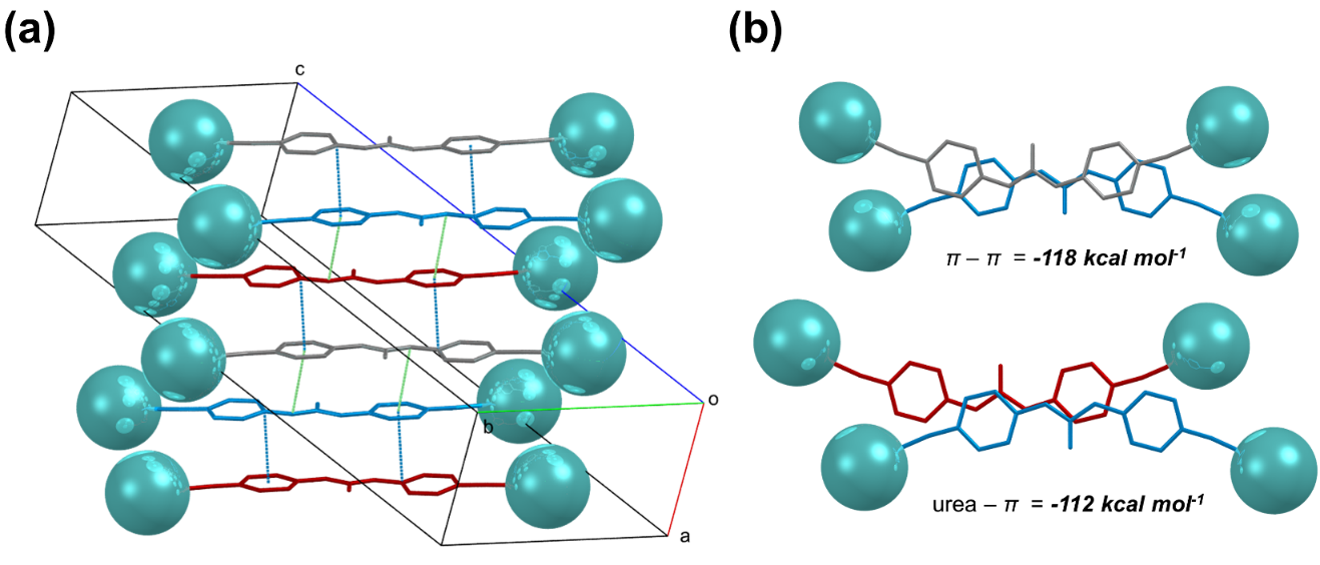
\includegraphics[width=0.8\linewidth]{figures/pub3/Picture7.png}
    \caption{\textbf{(a)} Solid-state packing of Mo(CO)$_{5}$-appended 1,3-bis(\textit{p}-isocyanophenyl)urea showing the orientation of the molecules relative to the unit cell axes. \textbf{(b)} Alternative representation viewed through the \textit{N,N'} diarylurea planes. All CO ligands and H atoms are omitted and Mo atoms are depicted at full Van der Waals radius (reproduced from CCDC 1905536) \citep{Millard2019a}}\label{fig:solid-state-packing}
\end{figure}

Based on the findings of the present and past works, we were inspired to extend our computational investigations to the crystal structure of an \textit{asymmetric} organometallic complex prepared by tethering a Mo(CO)$_{5}$ fragment to \textit{N}-(\textit{p}-isocyanophenyl)-\textit{N'}-phenylurea (\textit{p}Mo(CO)$_{5}$HDPU). Of primarily speculation, what are the principal interactions present, and are they consistent with the studied \textit{p}DPUs and/or the dioptic metal carbonyl complexes? Could the primary structural characteristics of the thermodynamically stable crystal be predicted from the knowledge gained through computational modeling of \textit{p}DPU crystallization behaviors? Again, the understanding of how to control the crystallization propensity of compounds synthesized comprising the versatile \textit{p}DPU moiety will guide our exploration into novel organometallic crystal systems with unique materials applications.


% FIGURE 8 
\begin{figure}[h!]
    \centering
    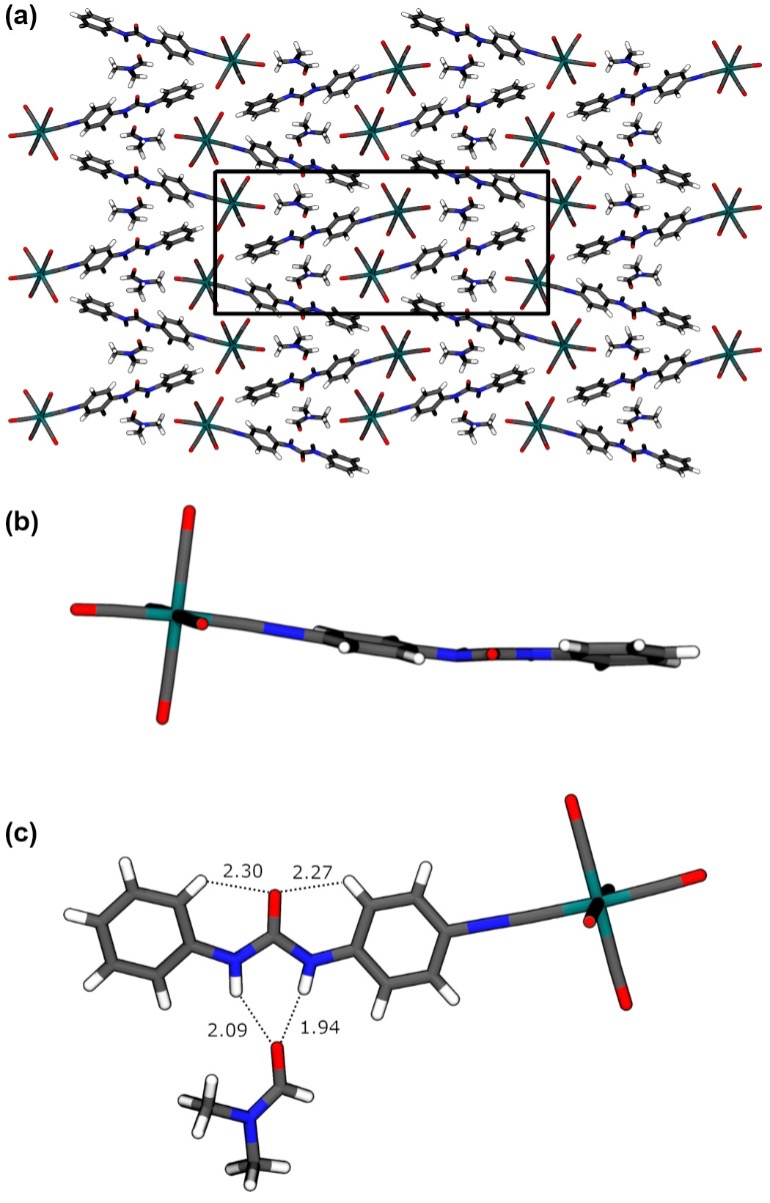
\includegraphics[width=0.8\linewidth]{figures/pub3/Picture8.jpg}
    \caption{\textbf{(a)} Molecular packing in the \textit{p}Mo(CO)$_{5}$HDPU crystal system. \textbf{(b)} Planar configuration of the \textit{p}DPU moiety as found in the \textit{p}Mo(CO)$_{5}$HDPU crystal structure. \textbf{(c)} Hydrogen bonding distances of \textit{o}-H$\cdot \cdot \cdot$O$_{urea}$ and H$_{urea}$$\cdot \cdot \cdot$O$_{DMF}$ contacts in the crystal structure.}\label{fig:mol-pack-MoCO5HDPU}
\end{figure}


Crystallographic characterization of the asymmetric \textit{p}Mo(CO)$_{5}$HDPU exhibited the \textit{p}DPU moiety crystallized in a nearly planar configuration despite the single asymmetric substitution, analogous to the \textit{p}NHDPU crystal structure (\autoref{fig:mol-pack-MoCO5HDPU}). This occurrence is likely due to the enhanced electron-withdrawing character of the Mo(CO)$_{5}$-CN$^{-}$ substituent as compared with the asymmetrically substituted \textit{p}CyHDPU, which exhibits the urea ribbon motif in the solid state. The bolstered electron-withdrawing nature of the metal carbonyl fragment provides the necessary intramolecular stabilization through \textit{o}-H$\cdot \cdot \cdot$O$_{urea}$ hydrogen bonding to maintain the planar molecular orientation in its crystalline configuration. Also akin to \textit{p}NHPDU was the co-crystallization of DMF solvent molecules at a 1:1 ratio. The DMF forms the stable H$_{urea}\cdot \cdot \cdot$O$_{DMF}$ hydrogen bonding complex in a likewise manner, thus filling otherwise void space created between the planar DPUs and bulky Mo(CO)$_{5}$ substituents, and adding additional stabilizing lattice energy. 

Based on the careful observations of the studied \textit{p}DPU systems, one may have predicted the observed nature of crystallization of the \textit{p}Mo(CO)$_{5}$HDPU molecule. The similar balance of intramolecular and intermolecular forces driving crystal nucleation and growth in the DPU crystal systems is met through the intricate interactions of the DPU moiety internally, with neighboring \textit{p}Mo(CO)$_{5}$HDPU molecules, and with the abundantly available solvent molecules. The resulting molecular conformations found in the isolated molecule and in the crystal structure are primarily consequences of the electron-withdrawing character of the DPU \textit{p}-substituents. Solvent molecules may or may not be incorporated into the crystal system based on spatial constraints and the energies associated with disrupting a preferred planar molecular conformation.

Remarkably, the Mo(CO)$_{5}$ moieties in crystalline \textit{p}Mo(CO)$_{5}$HDPU form an ordered array similar to that observed in the previously reported di-substituted 1,3-bis(\textit{p}-isocyanophenyl)urea. The distances between metal centers of \textit{p}Mo(CO)$_{5}$HDPU were 6.06, 6.85, and 8.18 \AA, which is remarkable close to those of the di-substituted species of 6.01, 6.87, and 7.58 \AA. This demonstrates the role in crystallization of the appended metal carbonyl fragments to the \textit{p}DPU structure. While the DPU elements behave in a seemingly predictable manner, the Mo(CO)$_{5}$ groups may as well. The result is the concerted balance between the two prominent molecular constituents that guides the formation of the supramolecular structure. Although the current sample size is limited for this specific class of molecular species, the convoluted balance of energies steering the nucleation and crystallization of complex solid-state systems may too become more predictable as we continue to gather data on such systems as this field of study progresses. 

We have established the role of \textit{p}DPUs in facilitating the growth of organic and organometallic crystal systems, and we have also shed light on the engagement of metal carbonyl fragments in patterning crystal growth. This study relies on quantum chemical calculations, experimental crystallographic analysis, and the chemical synthesis of a new class of organometallic complexes to improve the understanding of the intricacies of complex intra- and intermolecular interactions driving the formation of tailorable crystal structures with the hopes that this knowledge can be leveraged for predictive capabilities in the design of further novel materials. Continued perseverance and comprehensive computational and experimental investigations into DPU and organometallic derivatives may provide the necessary predictive ability for the engineering of novel crystal systems with enhanced performance in processing, development, and applications as charge-transfer materials.

\section{Conclusions}
Understanding the balance of opposing packing forces and conformational strain energies is paramount for the engineering of novel organic and organometallic crystalline materials. In this study, we categorize the intricate features of energetic contributions to the supramolecular assembly of \textit{p}-substituted \textit{N,N'}-diphenylureas (\textit{p}DPUs) and organometallic derivatives utilizing a holistic DFT approach. The results show a relationship between gas-phase and solid-state molecular conformations, and how the observed structural differences may or may not lead to deviations in expected crystallization behaviors based on the strengths of relative intra- and intermolecular interactions. Building on previous reports of DPU-based organometallic crystal systems, we also present the synthesis of an asymmetric Mo(CO)$_{5}$-substituted \textit{N}-(\textit{p}-isocyanophenyl)-\textit{N'}-phenylurea in efforts to further relate the crystallization behaviors and interactions of organometallic DPU derivatives with those of the base \textit{p}DPU systems. It was observed that the supramolecular assembly of the organometallic complexes display similar predictive crystallization patterns, as well as additional complexities evolving due to the bulky metal carbonyl substituents. We present a comprehensive computational classification of \textit{p}DPU-based crystal systems in complement to experimental data in our endeavors to develop reliable design rules for patterned crystal growth of DPU and related systems for the future generation of new materials having unique solid-state structures and properties.

\section{Acknowledgements}
We would like to acknowledge high-performance computing support of the R2 compute cluster (DOI: 10.18122/B2S4$^{1}$H) provided by Boise State University's Research Computing Department. 

\section{Supporting Information}
X-ray data collection and refinement parameters for \textit{p}Mo(CO)$_{5}$HDPU. (\autoref{chap:cataloguing_SI})

\section{Accession Codes}
CCDC 1554302, 676835, 1554299, 1554301, 676839, 1554300, 1905536, and 2035534 contain the supplementary crystallographic data for this paper. These data can be obtained free of charge from The Cambridge Crystallographic Data Centre at \url{www.ccdc.cam.ac.uk/data_request/cif} or by emailing \href{mailto:data_request@ccdc.cam.ac.uk}{data\_request@ccdc.cam.ac.uk}.
